\subsection{Fundamentals of Fixed Income}

\begin{figure}[H]
\centering
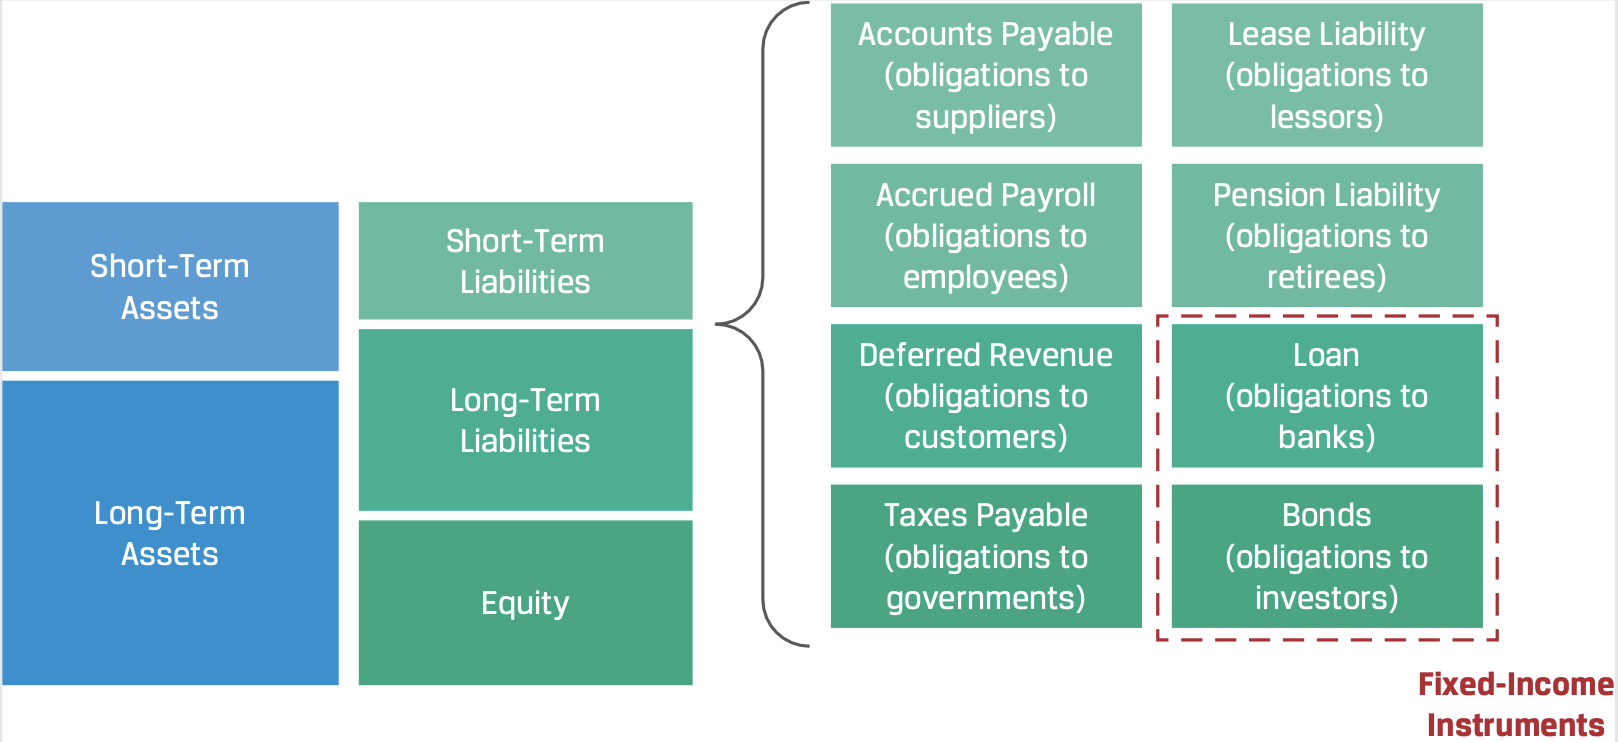
\includegraphics[scale=0.4]{/fi/fiscope}
\caption{Scope of fixed income instruments}
\end{figure}

\begin{remark} Issuers of Fixed Income
\begin{enumerate}[label=\roman*.]
\setlength{\itemsep}{0pt}
\item Supranational Organisations: World Bank, European Bank
\item Government Bonds: sovereign (national), non-sovereign (local), quasi-national (agencies)
\item Corporate: from financial and non-financial firms
\item Special Legal Entities: securitise assets for asset-backed securities (ABS)
\end{enumerate}
\end{remark}

\begin{remark} Common Terminology
\begin{enumerate}[label=\roman*.]
\setlength{\itemsep}{0pt}
\item Maturity: date of final payment the issuer makes to investors
\item Tenor: remaining time to maturity
\item Par Value: amount issuer agrees to pay the bondholder on the maturity date, quoted on $100$-point system
\item Market Reference Rate: standard borrowing or lending rate for issuers with lowest default risk for different currencies and maturities.
\end{enumerate}
\end{remark}

\begin{remark} \hlt{Classification of Fixed Income by Maturity}
\begin{enumerate}[label=\roman*.]
\setlength{\itemsep}{0pt}
\item Money Market Security: maturity at issuance less than $1$ year
\item Capital Market Security: maturity at issuance greater than $1$ year
\item Perpetual Bonds: bond type with no stated maturity
\end{enumerate}
\end{remark}

\begin{remark} \hlt{Classification of Fixed Income by Coupon Rate and Frequency}
\begin{enumerate}[label=\roman*.]
\setlength{\itemsep}{0pt}
\item Floating-Rate Notes (FRNs): market reference rate (MRR) with issuer-specific credit spread.
\item Quarterly Income Debt Security (QUIDS): senior unsecured debt issued in small denominations with long maturities, interest paid quarterly.
\end{enumerate}
\end{remark}